\chapter{Forschungsstand}
\label{chap:forschungsstand}
Seit den Anfängen der Entwicklung von \gls{open-ran} im Februar 2016 und der Gründung von \gls{oran} 2018 gibt es einige wissenschaftliche Arbeiten, die sich mit dem Thema Schwachstellenanalyse und Schwachstellenbewertung in einer \gls{open-ran} Umgebung beschäftigen. Auch in anderen Feldern der Informatik werden empirische Methoden genutzt, um die Sicherheit von Komponenten im jeweiligen System zu analysieren und bewerten. In diesem Kapitel wird ein Überblick über den Forschungsstand anhand einer Auswahl von Arbeiten gegeben \autocite{Us} \autocite{GuideOpenRAN}.
%
\section{\citetitle{o-ranworkgroup11securityworkgroupORANSecurityThreat2024} - O-RAN WG11}
\label{sec:forschungsstand-wg11}
Die \gls{wg11} der \gls{oran} beschäftigt sich mit den sicherheitstechnischen Aspekten von \gls{open-ran} und veröffentlicht in regelmäßigen Abständen einen technischen Report, der eine Bedrohungsmodellierung und Risikobeurteilung enthält. Zum Zeitpunkt der Veröffentlichung ist der Report in Version \textit{\textsf{v04.00}} die neuste Fassung dieses Dokuments. Der Report umfasst sowohl mögliche Angriffe auf Komponenten in einem \gls{oran}-System, als auch nicht \gls{oran} spezifische Bedrohungen, wie Supply-Chain-Angriffe auf Quell-Offenen Programmcode oder physischen Eingriff um auf sensible Daten zu erlangen\autocite{o-ranworkgroup11securityworkgroupORANSecurityThreat2024}. Der Einfachheit halber wird im Folgenden nur auf die \gls{oran}-spezifischen Bedrohungen eingegangen. Die betroffenen Komponenten sind in Abbildung \ref{fig:oran-architecture} dargestellt. Die \gls{wg11} identifiziert dazu 35 Bedrohungen in der Komponente \textit{O-RAN Cloud} und 69 Bedrohungen die auf alle anderen Komponenten zutreffen \autocite[Seite 31 - 69]{o-ranworkgroup11securityworkgroupORANSecurityThreat2024}.
\par Der Großteil der Bedrohungen wird dabei in der Risikobewertung mit einem Risikowert von \textit{High} eingestuft, vgl. Abbildung \ref{fig:riskscore-oran-components} \autocite[Seite 130 - 164]{o-ranworkgroup11securityworkgroupORANSecurityThreat2024}.
%
\begin{figure}[H]
    \centering
    \label{fig:riskscore-oran-components}
    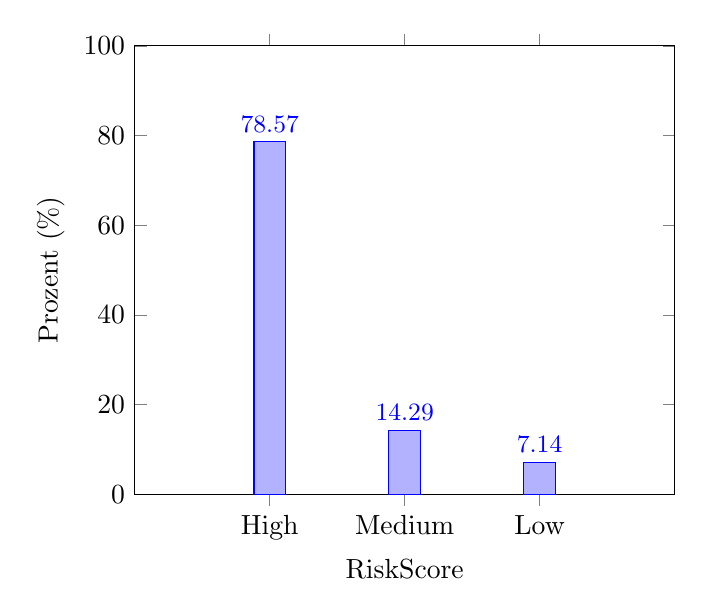
\begin{tikzpicture}
        \begin{axis}[
            ybar,
            symbolic x coords={High, Medium, Low},
            xtick=data,
            ymin=0, ymax=100,
            ylabel={Prozent (\%)},
            xlabel={RiskScore},
            nodes near coords,
            every node near coord/.append style={font=\small},
            bar width=0.4cm,
            enlarge x limits=0.5
        ]
        \addplot coordinates {(High, 78.57) (Medium, 14.29) (Low, 7.14)};
        \end{axis}
    \end{tikzpicture}
    \caption{Risikobewertung der Bedrohungen in der O-RAN Komponenten}
\end{figure}
%
\section{\citetitle{kopsellOpenRANRisikoanalyse2022} - \citeauthor{kopsellOpenRANRisikoanalyse2022}}
\label{sec:forschungsstand-bsi}
In dieser Studie wird eine weitere Risikoanalyse durchgeführt. Diese Studie ist im Gegensatz zu \ref{sec:forschungsstand-wg11} von einer externen Organisation, der secunet Security Networks AG, beauftragt und finanziert vom \gls{bsi}, durchgeführt worden. \citeauthor{kopsellOpenRANRisikoanalyse2022} führen an, dass die veröffentlichten \gls{oran}-Spezifikationen zum Zeitpunkt Februar 2022 nicht viele Vorgaben zur Sicherheit machen und sich insbesondere nicht an dem Ansatz \textit{security/privacy by design/default} orientiert. Als Folge dessen werden viele Sicherheitsrisiken mit mittlerem bis hohem Schweregrad festgestellt.
\par Weitere umfangreiche Risikoanalysen für 5G oder 5G RAN wurden von \gls{nis} und \gls{enisa} veröffentlicht, diese sind aber nicht auf \gls{open-ran} fokussiert \autocite{europeanunionagencyfornetworkandinformationsecurity.ENISAThreatLandscape2019} \autocite{EUCoordinatedRisk}.
%
\section{\glqq{}ACEMA\grqq{} - \citeauthor{klementSecuring6GTransition2024}}
\label{sec:forschungsstand-acema}
\citeauthor{klementSecuring6GTransition2024} untersuchen in ihrem Artikel \citetitle{klementSecuring6GTransition2024} die Sicherheitsherausforderungen, die mit dem Übergang von 5G zu 6G-Netzen und der Einführung von \gls{open-ran}-Technologien einhergehen. Ziel ihrer Forschung ist die Entwicklung eines umfassenden Ansatzes zur Bewertung und Priorisierung von Sicherheitsbedrohungen in Open-RAN-Umgebungen, wobei die O-Cloud-Komponente als repräsentatives Beispiel dient. Hierzu kombinieren die Autoren das \gls{mitre} ATT\&CK Framework mit empirischen Daten, um spezifische Bedrohungen in einer O-RAN-Implementierung zu analysieren und effektive Gegenmaßnahmen abzuleiten. Im Zentrum ihrer Methodik steht die Abbildung einer \gls{mitre}-Technik zu einem spezifischen CVE-Datum über das Durchsuchen der unterschiedlichen Kategorisierungssysteme \gls{capec}, \gls{cwe} und \gls{cve}. Die Anwendung eines Bewertungssystems, das auf dem \gls{cvss} basiert, um den Schweregrad möglicher Schwachstellen zu bewerten, geht über die bisher vorgenommenen Bewertungssysteme der \gls{oran} Alliance heraus und ermöglicht eine granuläre Auswertung der Ergebnisse. Die Erkenntnisse dieser Arbeit tragen dazu bei, die Sicherheitslücken in Open RAN zu minimieren, indem Bewusstsein für spezifische Bedrohungsszenarien geschaffen wird. Dies wird durch einfach verständliche Datenvisualisierungen unterstützt.
\par Die Veröffentlichung von \citeauthor{klementSecuring6GTransition2024} spielt, wie bereits in Kapitel \ref{chap:Einleitung} erwähnt, für diese Abschlussarbeit eine wichtige Rolle. Die Modularität des Ansatzes erlaubt eine Übertragung auf verschiedene Komponenten \autocite{klementSecuring6GTransition2024}.

%
\section{\citetitle{mazuera-rozoAndroidOSStack2019} - \citeauthor{mazuera-rozoAndroidOSStack2019}}
\label{sec:forschungsstand-android}
Im Umfeld von Android wurde eine empirische Studie durchgeführt die, ähnlich wie \gls{acema} im Umfeld von \gls{open-ran}, eine umfangreiche Schwachstellenanalyse und Schwachstellenbewertung auf allen öffentlich auffindbaren Schwachstellen betrachtet. \citeauthor{mazuera-rozoAndroidOSStack2019} betrachten in dieser Studie besonders die Art der Schwachstellen und wie sich diese über den Verlauf der Zeit ändern, die Angriffsvektoren nach \gls{cvss}, die angegriffenen Ebenen und Teilsysteme von Android und wie lange es dauert, bis die Schwachstellen geschlossen werden. Die Studie nutzt die \gls{mitre} \gls{cwe} Kategorisierung um die spezifischen Schwachstellen\footnote{\textit{Englische Übersetzung}: vulnerabilities} einer übergeordneten Schwachstelle\footnote{\textit{Englische Übersetzung}: weakness} zuzuordnen. Sie kommen zu dem Schluss, dass die meisten Schwachstellen eine schwere Auswirkung auf die Vertraulichkeit, Integrität und Verfügbarkeit des Geräts haben \autocite{mazuera-rozoAndroidOSStack2019}. Eine ähnliche Datenanalyse, wie in \cite[Abbildung 10 (a)]{mazuera-rozoAndroidOSStack2019} die Angriffsvektoren auf \gls{cwe}'s darstellt, ist auch mit \gls{acema} möglich \autocite{klementSecuring6GTransition2024}.